\documentclass[11pt]{article}
\usepackage{times}
\usepackage{graphicx}
\usepackage{amsmath}

\begin{document}

\centerline{\sc \large Project Progress Report}
\vspace{.5pc}
\centerline{\sc Team Name: Yet Another Layer [YAL]}
\centerline{\sc Team Members: Cameron Fabbri, MD Jahidul Islam}
\centerline{\sc 3/27/2017}
\vspace{2pc}

\centerline{\sc \large Generative Adversarial Networks for Automatic Image Colorization }

\section{Objectives}
Our objectives given in the project proposal are stated below. 

\noindent (1) Implement the state of the art[1] for image colorization. \newline
\noindent (2) Implement Deep Convolutional Generative Adversarial Networks (DCGANs)[3]. \newline
\noindent (3) Implement Energy-Based Generative Adversarial Networks (EBGANs).[2] \newline
\noindent (4) Explore methods to pretrain the model used in 1 and fine tune it as a generator in 2 and 3.
\newline
\noindent (5) Time permitting, develop our own GAN architecture for comparison. \newline

\noindent Jahidul: 1, 4, 5 \newline
\noindent Cameron: 2, 3, 5 \newline

\noindent Cameron has implemented an adversarial network similar to the architecture used in [6]. Our model
is capable of using a combination of multiple loss functions. These include the typical L1 and L2 losses,
as well as various types of adversarial losses, such as the Wasserstein GAN [7] and the Least Squares GAN
[8].
\vspace{1pc}

\noindent Jahidul has implemented the Colorful Colorization network shown in [1] using L2 and L1 loss function. The original paper also implemented their own loss function, which is a major contribution to their work. Jahidul is currently implementing that loss function. We expect an improved colorization performance of the model using their customized loss function. 
\vspace{3mm}

\noindent Both of these have been trained and tested on the CelebA dataset [5]. Samples are shown below.
The different type of GAN Methods shown are as follows. GAN follows the loss as described in [4],
Wasserstein follows the loss as described in [7], and Least Squares follows the loss described in [8]. The
final loss for each model is informally $(GAN Weight \times GAN Method) + (L1 Weight \times L1 Loss) +
(L2 Weight \times L2 Loss)$

\begin{figure*}[t]
\vspace{-10mm}
\hspace{-25mm}
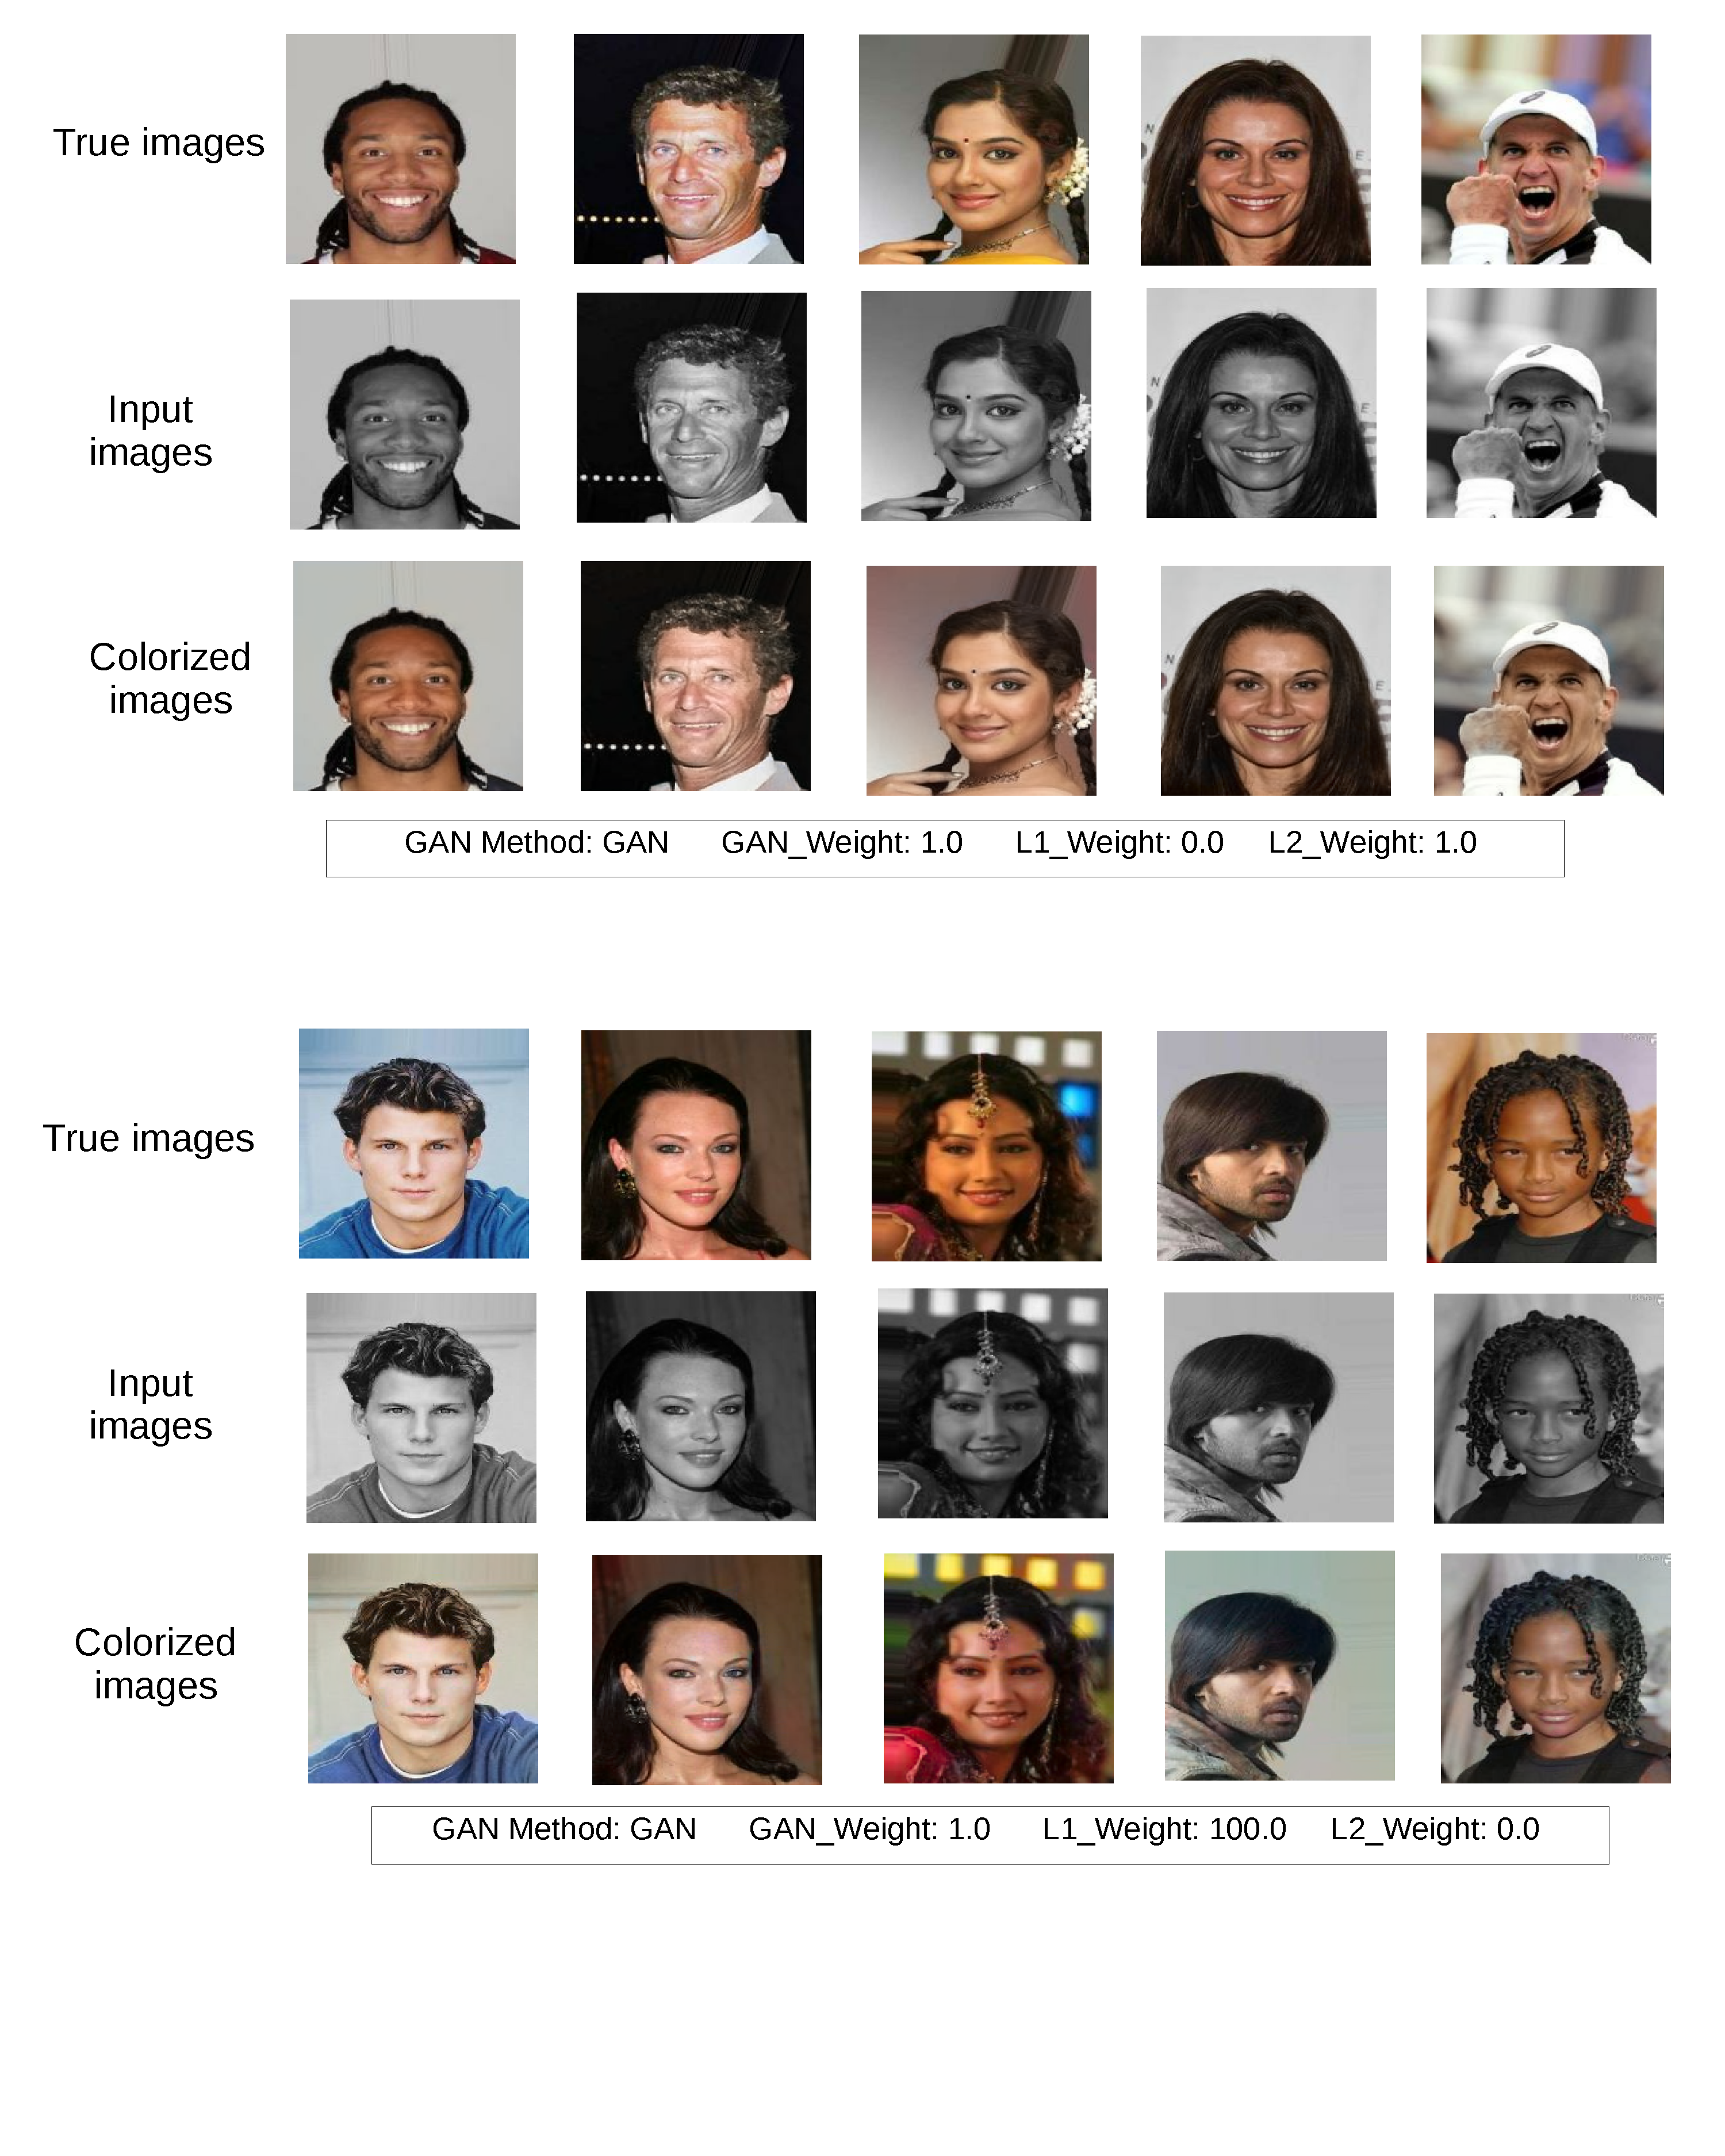
\includegraphics [scale=0.32]{1.pdf}
\vspace{-26mm}
\caption{Results for colorization with different models}
%\vspace{-5mm}
\label{fig:1}
\end{figure*}

\begin{figure*}[t]
\vspace{-10mm}
\hspace{-20mm}
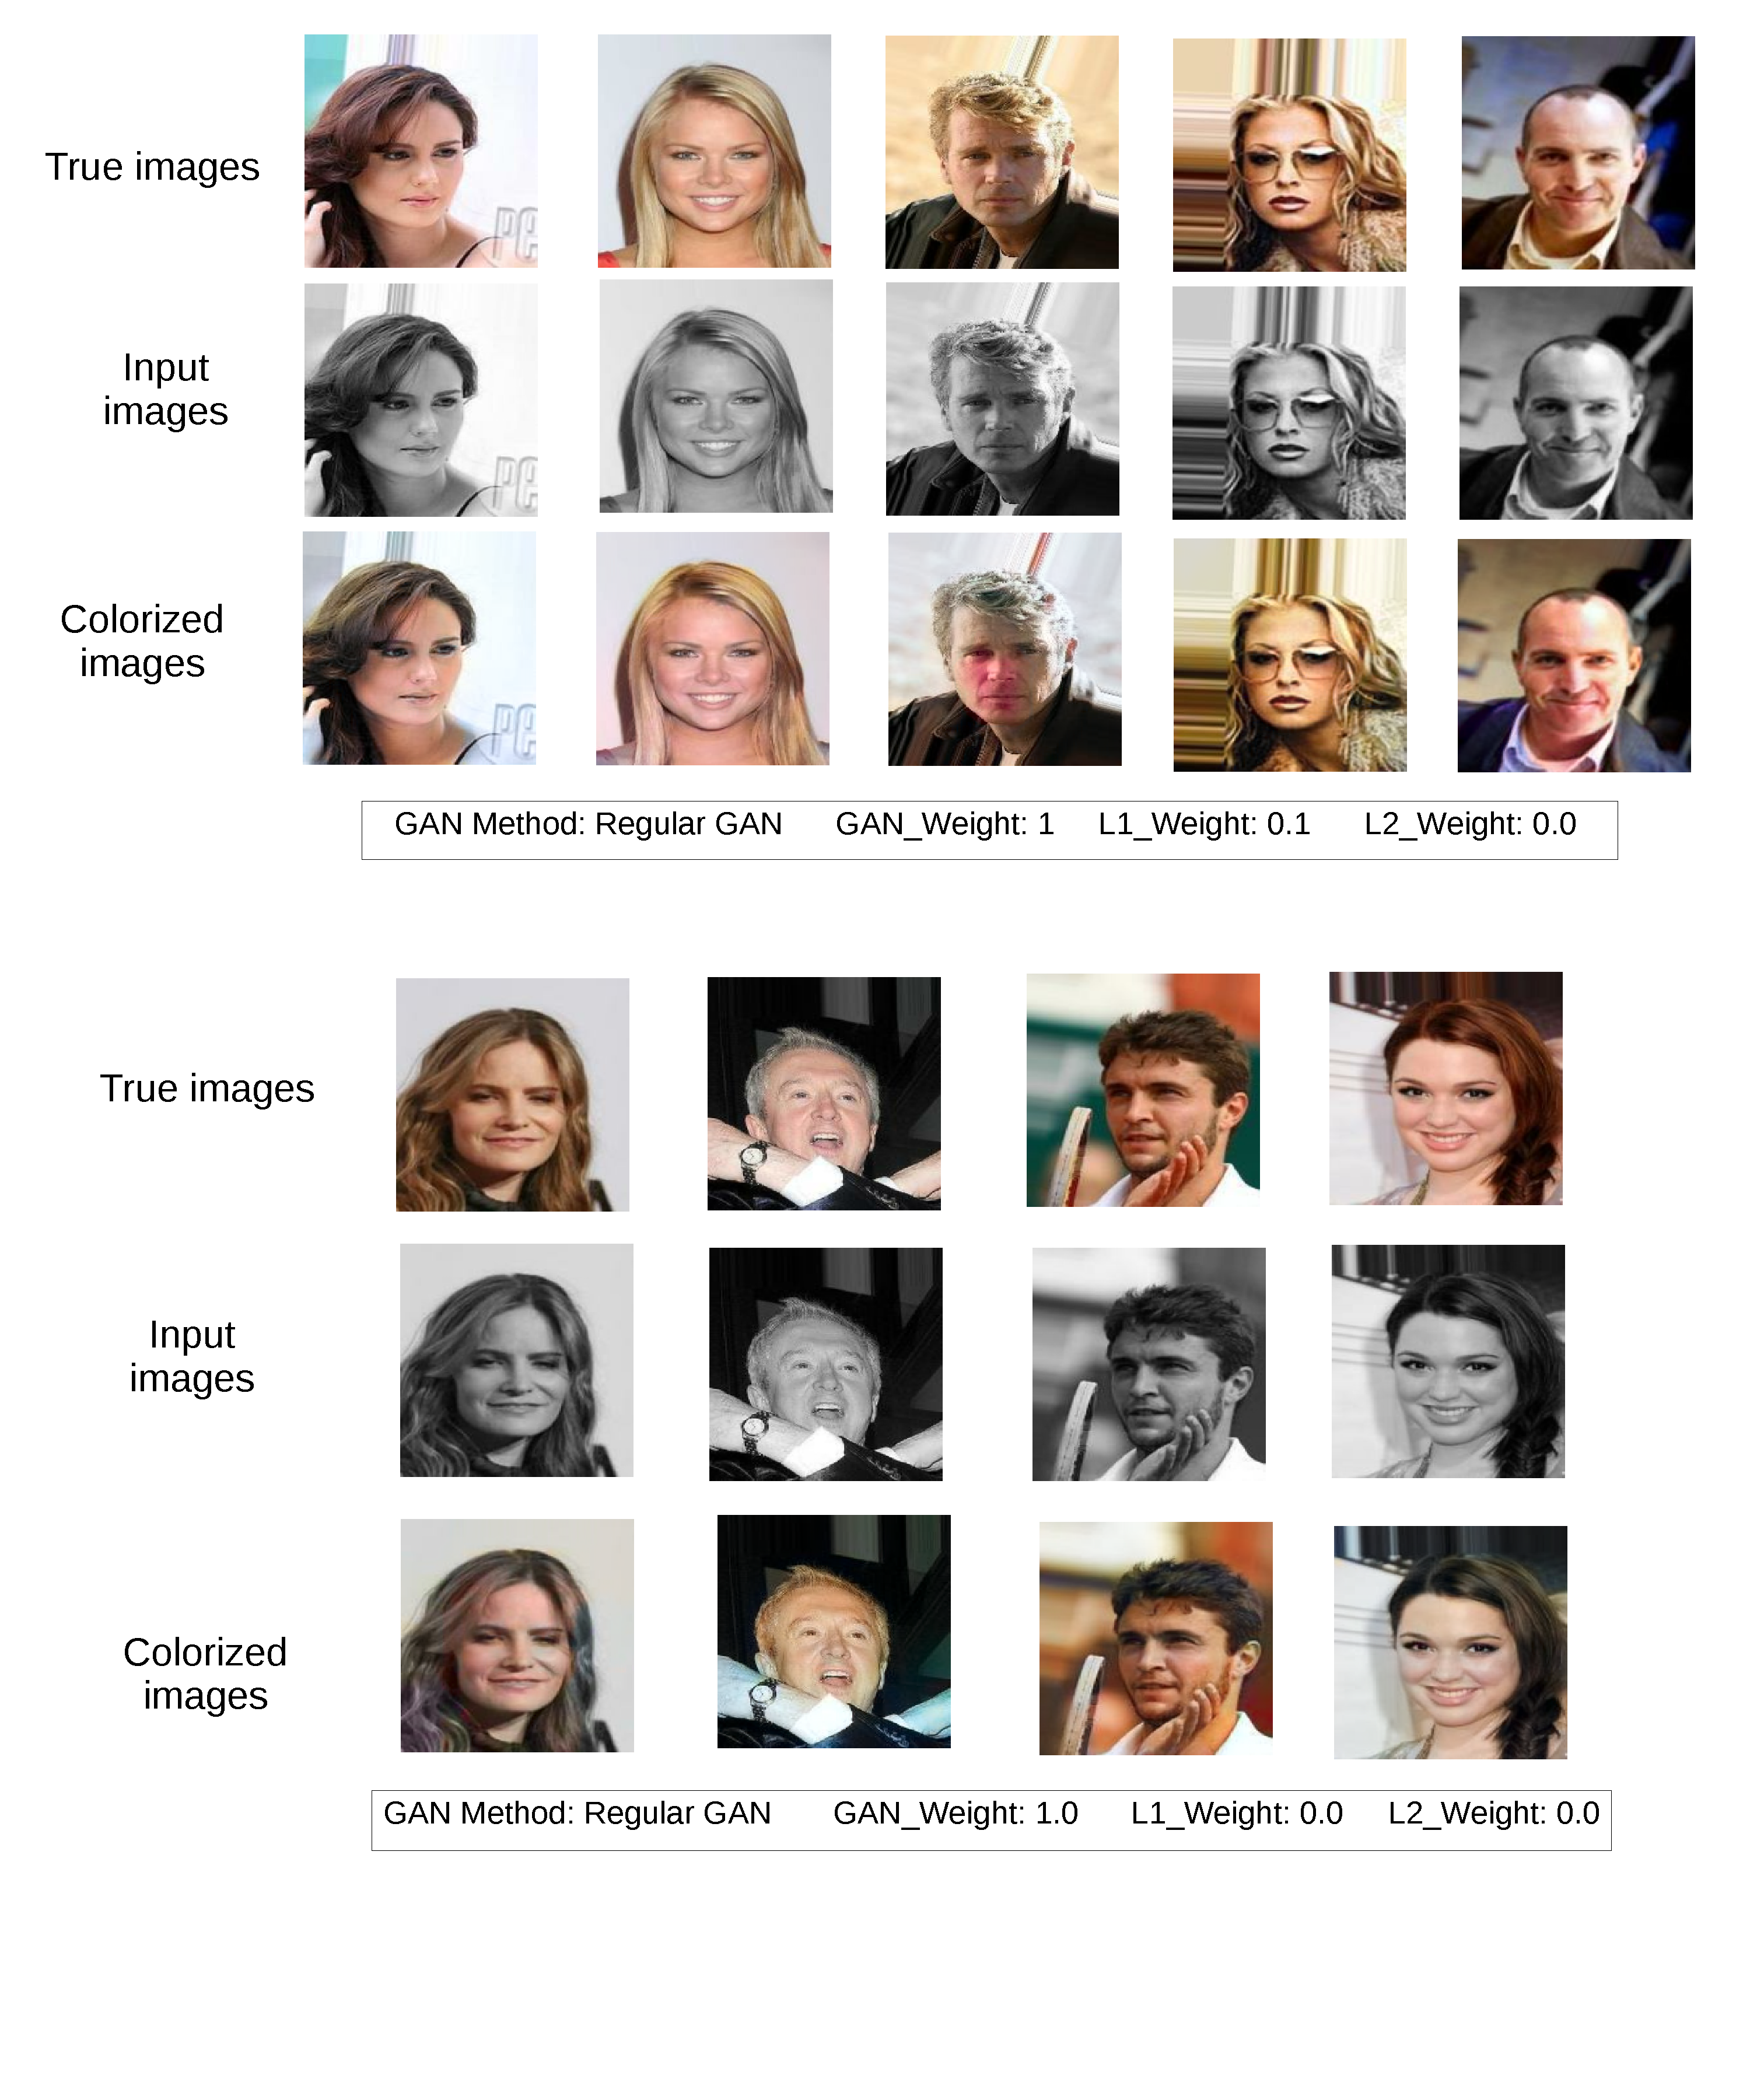
\includegraphics [scale=0.34]{2.pdf}
\vspace{-16mm}
\caption{Results for colorization with different models (contd.)}
%\vspace{-5mm}
\label{fig:2}
\end{figure*}

\begin{figure*}[t]
\vspace{-10mm}
\hspace{-20mm}
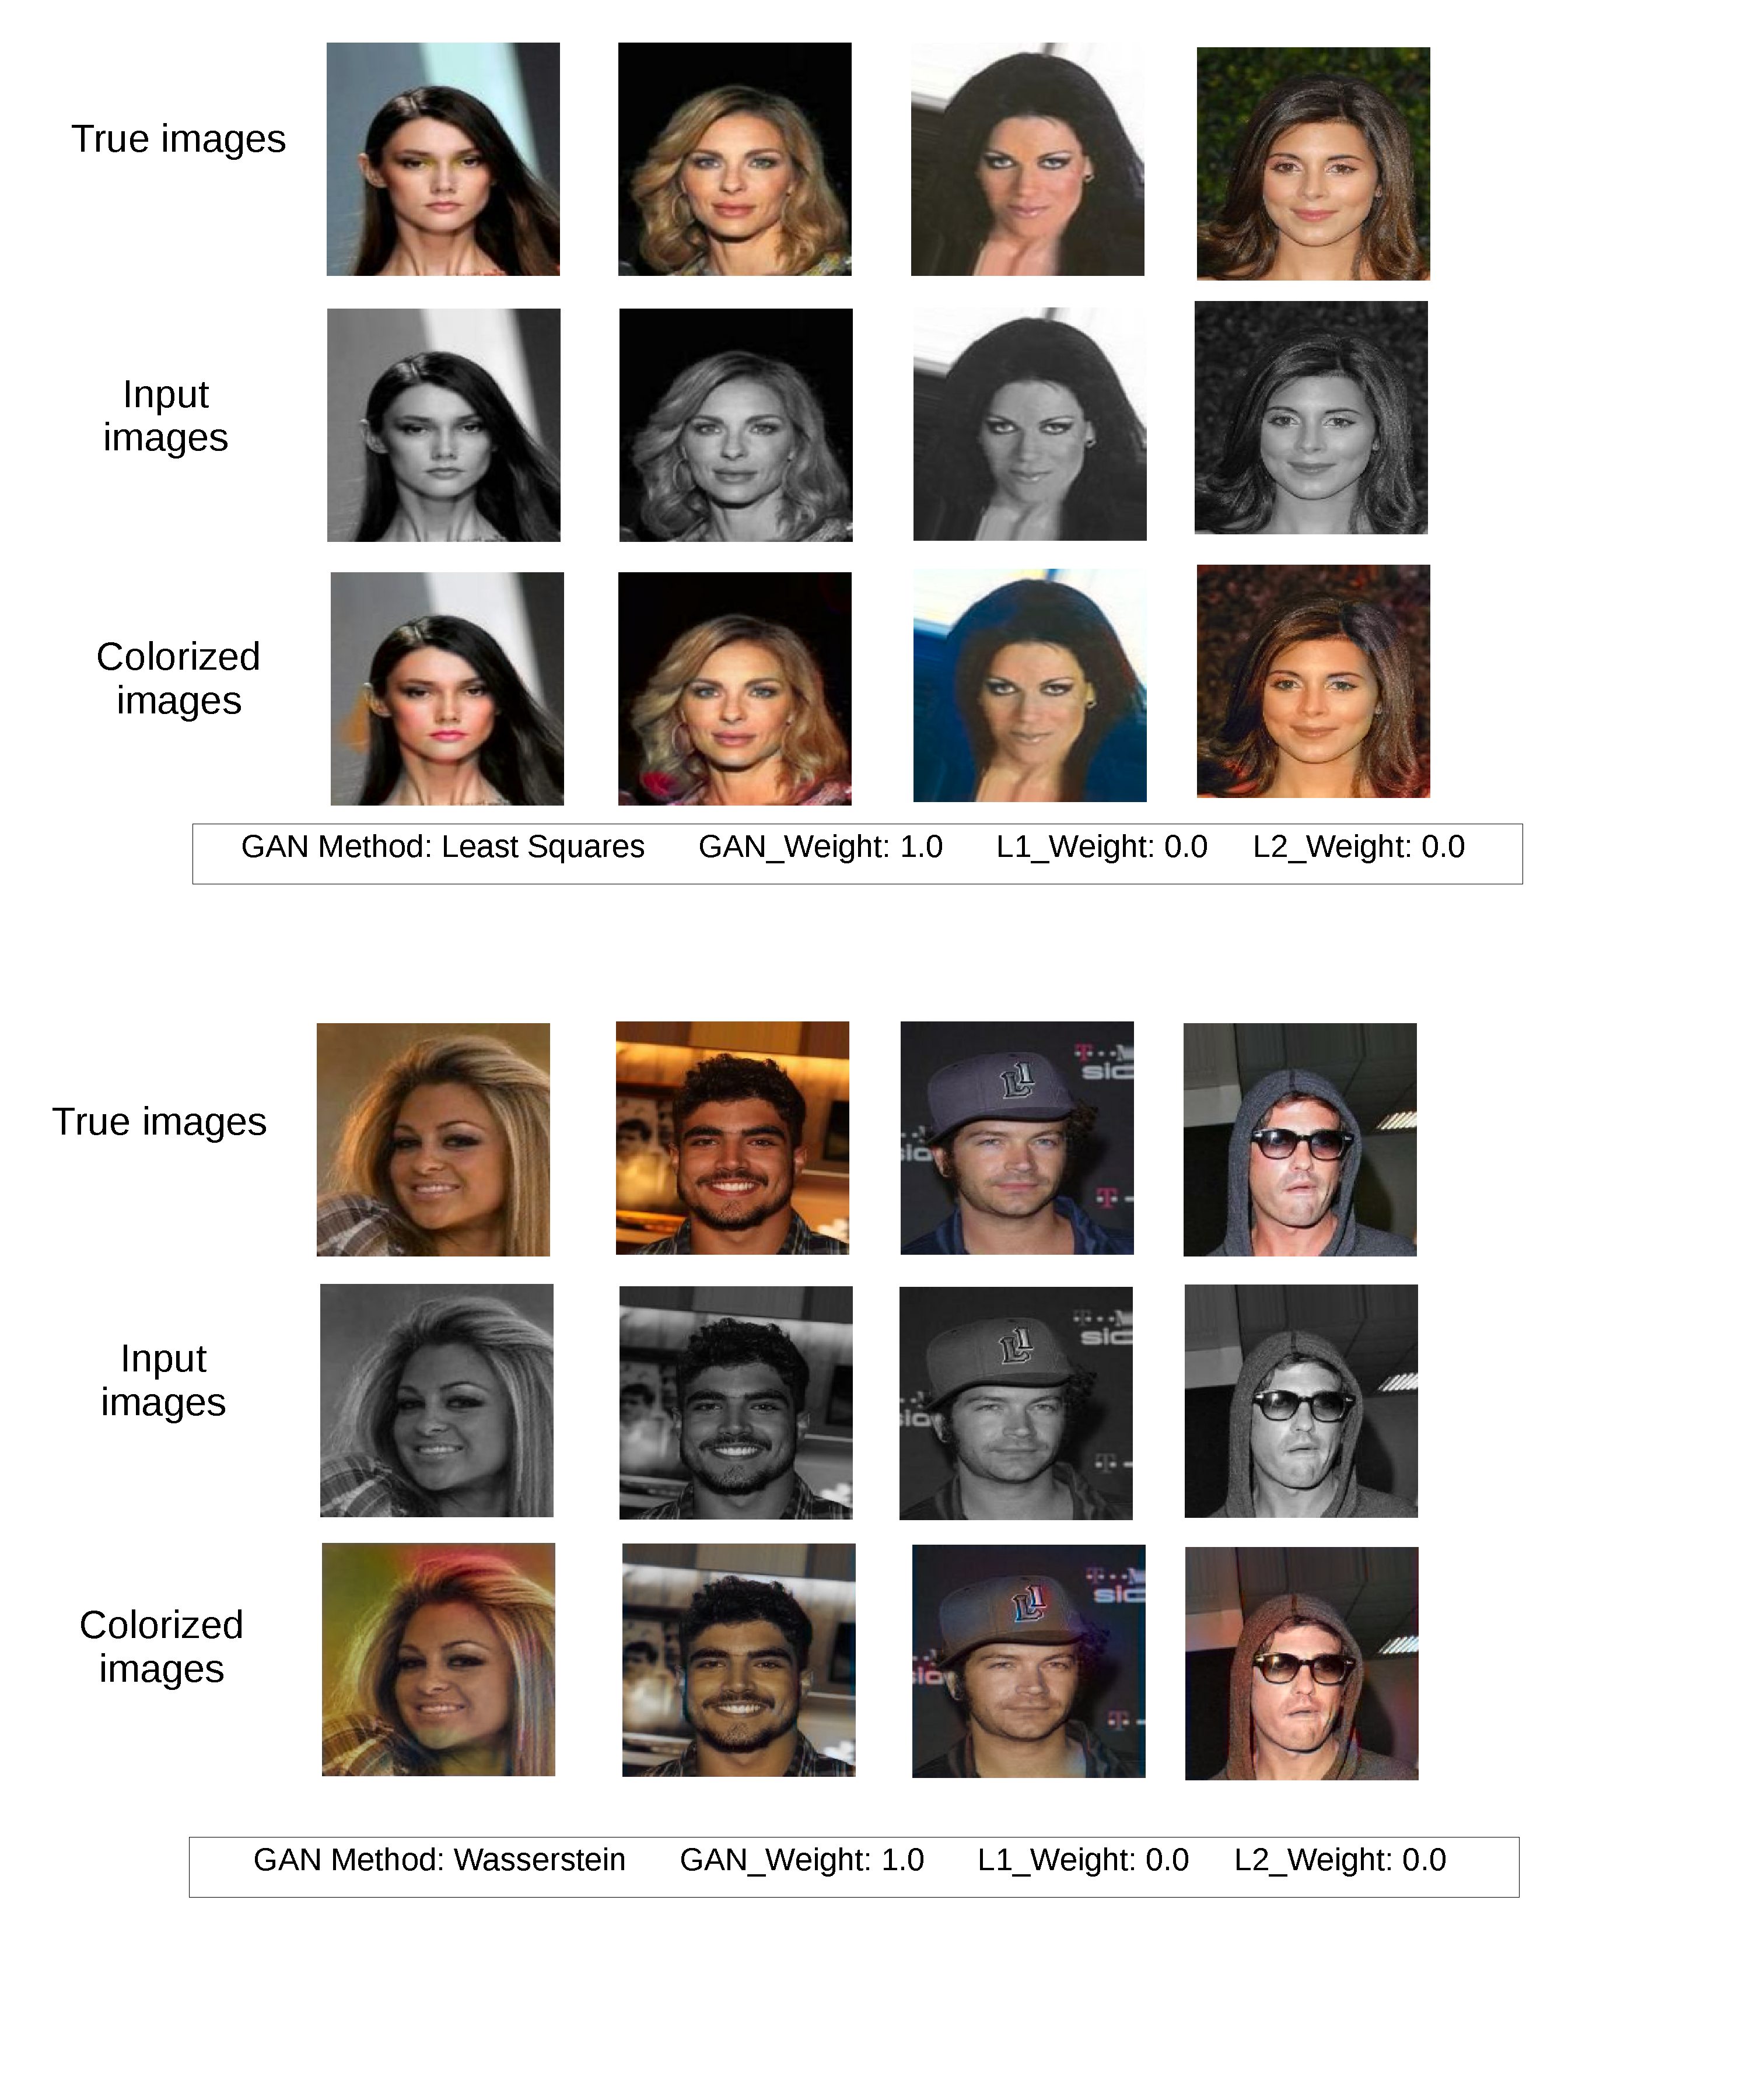
\includegraphics [scale=0.34]{3.pdf}
\vspace{-16mm}
\caption{Results for colorization with different models (contd.)}
%\vspace{-5mm}
\label{fig:2}
\end{figure*}

\begin{figure*}[t]
\vspace{-10mm}
\hspace{-20mm}
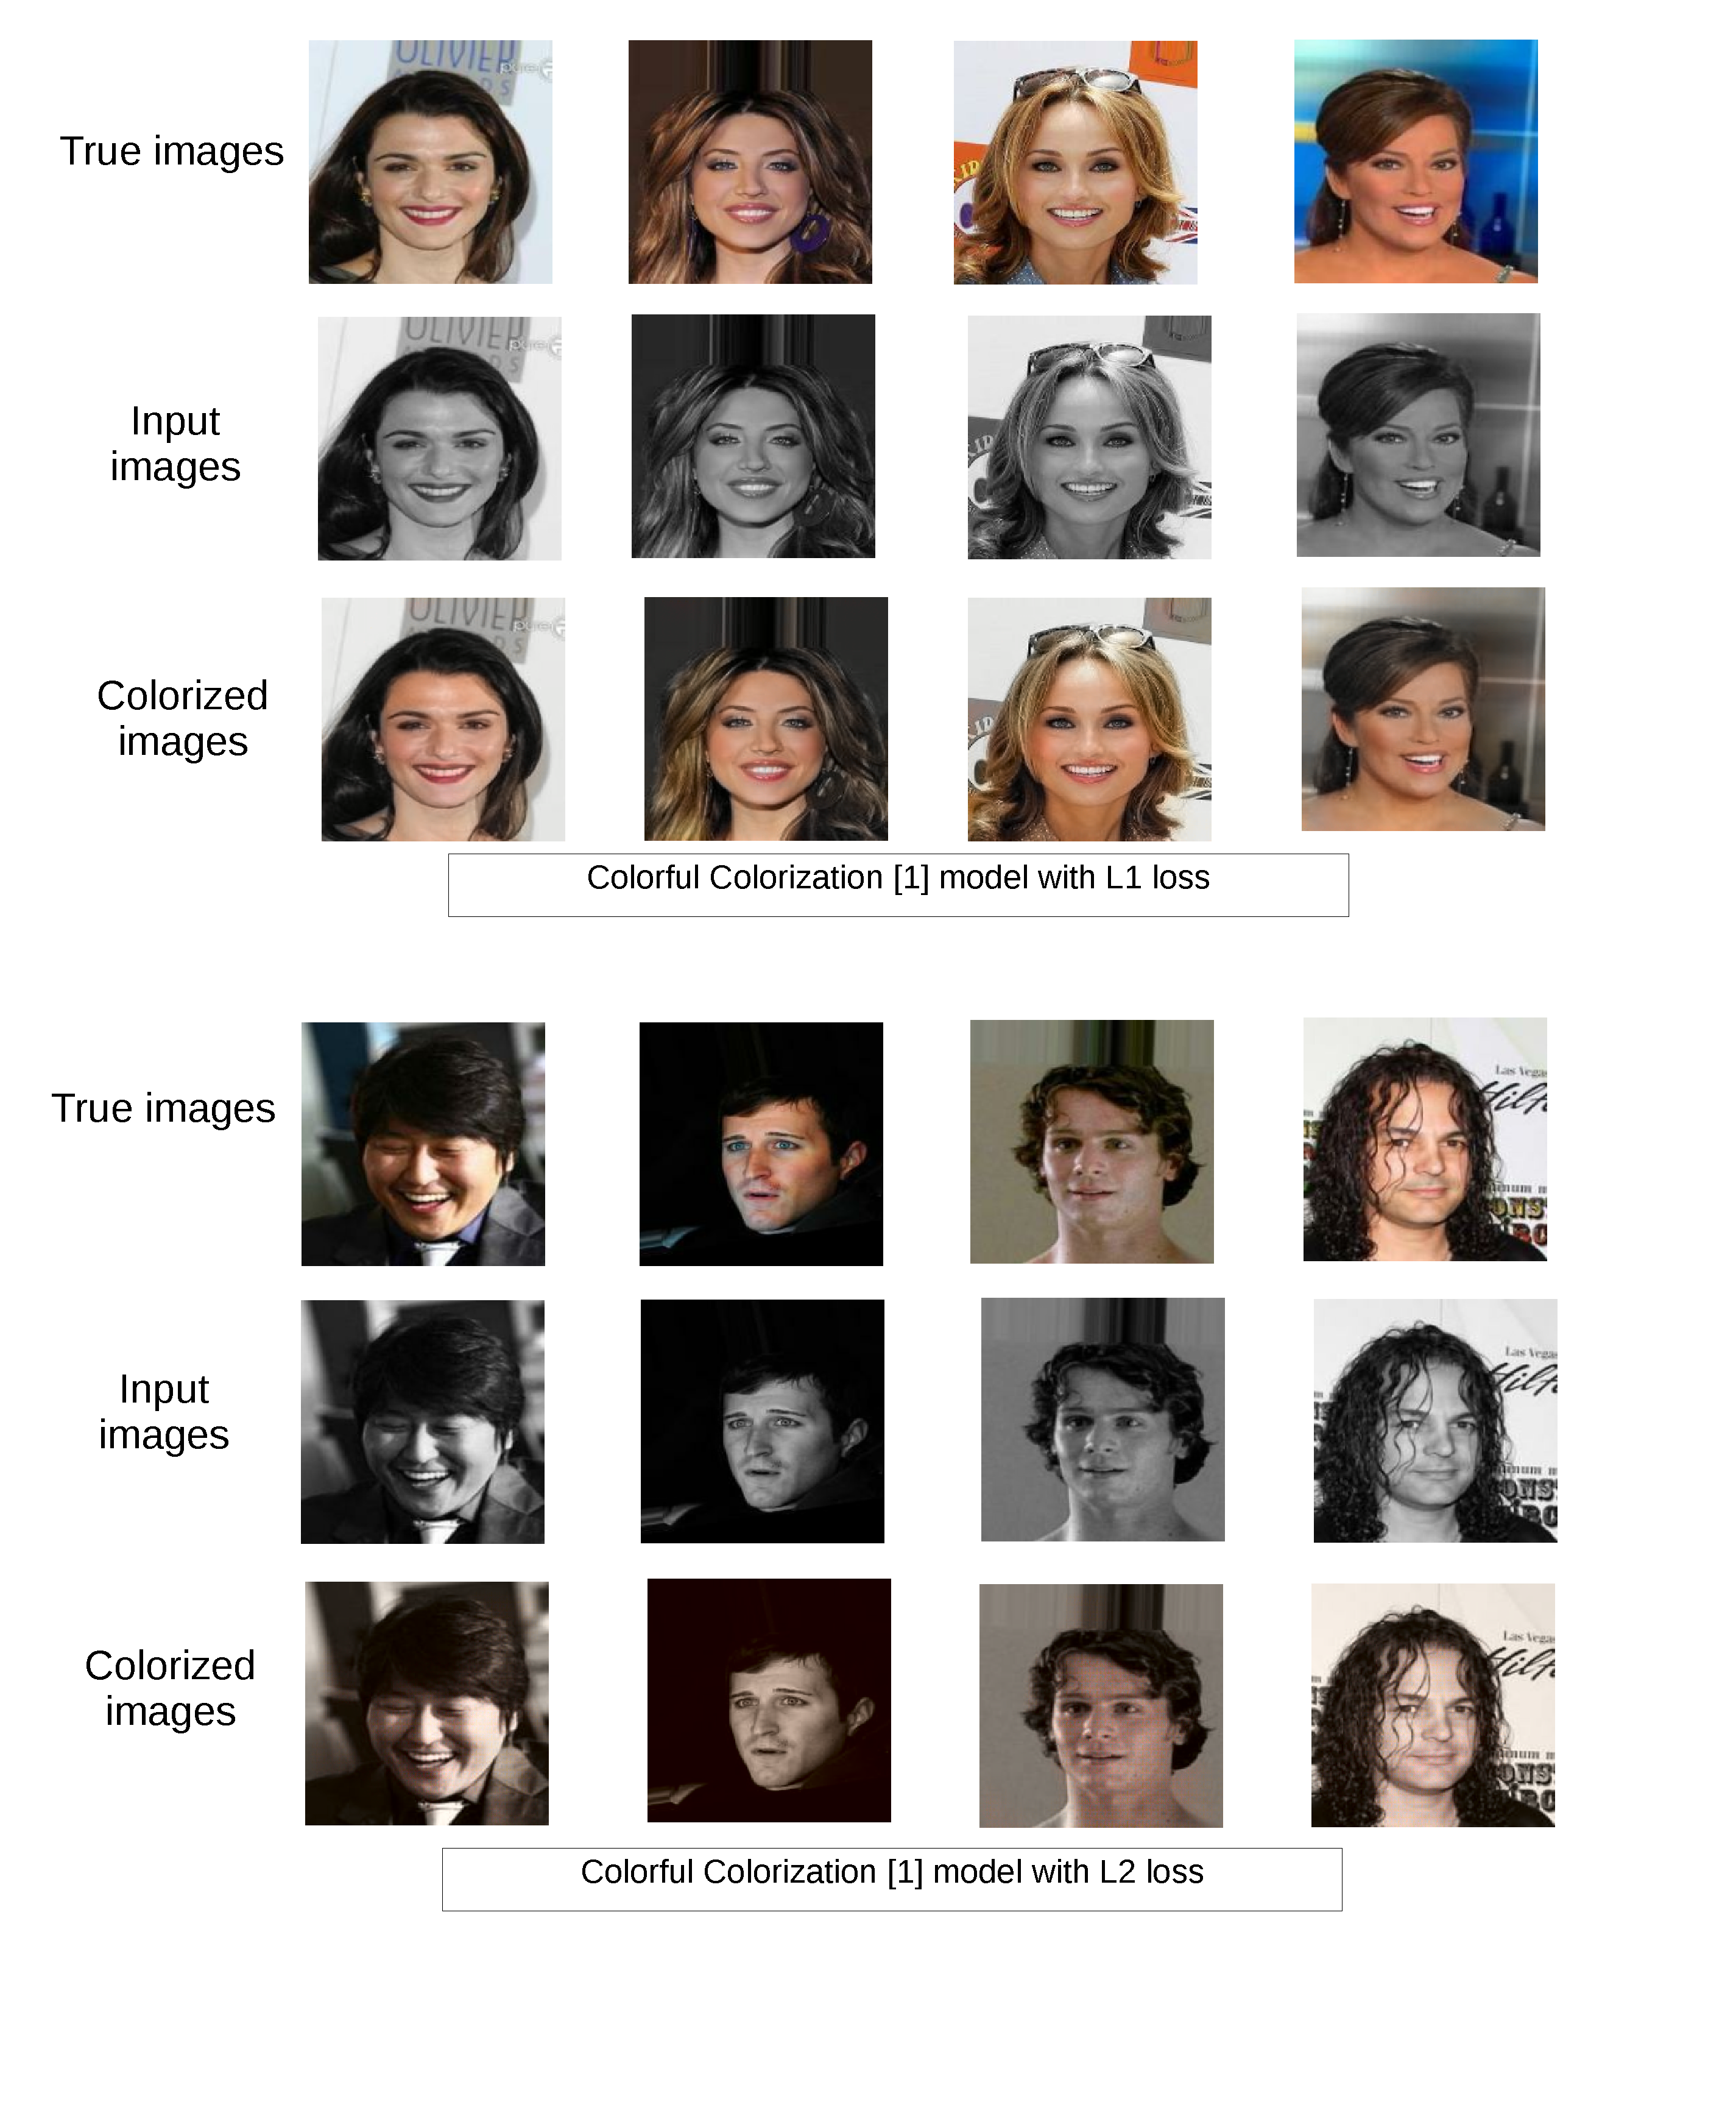
\includegraphics [scale=0.35]{4.pdf}
\vspace{-18mm}
\caption{Results for colorization with different models (contd.)}
%\vspace{-5mm}
\label{fig:2}
\end{figure*}

\newpage
\section{To Do}
We still have a number of things to test, such as pretraining the generator, implementing Energy-Based GANs,
combining the loss function in [1] with GAN loss, and training on multiple classes. While some of our results
show good performance on one class, we are uncertain how this will scale to multiple classes. Another
idea we are considering is, given the number of different combinations of L1 and L2 weights that can be
used with the GAN loss, we are thinking that given a perfect discrimator, the weights of L1 and L2 can be
treated as trainable parameters, and optimized in order to fool the discriminator.



\section{References}
[1] Zhang, Richard, Phillip Isola, and Alexei A. Efros. "Colorful image colorization." 
European Conference on Computer Vision. Springer International Publishing, 2016.
\vspace{2pt}

\noindent [2] J. Zhao, M. Mathieu, and Y. LeCun.  Energy-based Generative Adversarial 
Network. ArXiv e-prints, September 2016.
\vspace{2pt}

\noindent [3] Radford, Alec, Luke Metz, and Soumith Chintala. "Unsupervised representation learning with deep
convolutional generative adversarial networks." arXiv preprint arXiv:1511.06434 (2015).

\noindent [4] Goodfellow, Ian, et al. "Generative adversarial nets." Advances in neural information processing systems. 2014.

\noindent [5] Liu, Ziwei, et al. "Deep learning face attributes in the wild." Proceedings of the IEEE International Conference on Computer Vision. 2015.

\noindent [6] Isola, Phillip, et al. "Image-to-image translation with conditional adversarial networks." arXiv preprint arXiv:1611.07004 (2016).

\noindent [7] Arjovsky, Martin, Soumith Chintala, and Léon Bottou. "Wasserstein gan." arXiv preprint arXiv:1701.07875 (2017).

\noindent [8] Mao, Xudong, et al. "Least Squares Generative Adversarial Networks." arXiv preprint arXiv:1611.04076 (2016).


\end{document}
